%!TEX root = ../thesis.tex
\begin{savequote}[75mm]
Nulla facilisi. In vel sem. Morbi id urna in diam dignissim feugiat. Proin molestie tortor eu velit. Aliquam erat volutpat. Nullam ultrices, diam tempus vulputate egestas, eros pede varius leo.
\qauthor{Quoteauthor Lastname}
\end{savequote}

\chapter{Results}
\label{chap:results}

\newthought{Several experiments} were designed to evaluate the performance of the Discrete Voter Model. Two case studies, on elections in Chicago, were chosen to demonstrate DVM's performance on real data.

\section{Experiment Specification}
\label{sec:exper_spec}

The Discrete Voter Model was evaluated on the $2 \times 2$ case (i.e. $2$ candidates and $2$ demographic groups) and the $3 \times 2$ case that was untenable for previous methods of determining racially polarized voting.

The Discrete Voter Model was run on mock \texttt{Election} created with the specifications in Subsections \ref{subsec:two_by_two} and \ref{subsec:three_by_two}, using \texttt{dvm\_evaluator}. All other variables are in Table \ref{table:dvm_vars}.

\begin{table}[ht]
 \centering
 \caption{Non-Election Variables for DVM Experiments}
 \label{table:dvm_vars}
 \begin{tabular}{|l|c|c|}
   \hline
   \multicolumn{1}{|c}{Variable} & \multicolumn{1}{|c|}{option $1$}& \multicolumn{1}{c|}{option $2$} \\
   \hline
   number of MCMC steps, $t$ & $1000$ & $10000$ \\
   granularity of the PHCs, $g$ & $10$ & $100$ \\
   scoring function & \texttt{expec\_votes} & \texttt{prob\_votes} \\
   kernel & Random Walk Metropolis & Hamiltonian Monte Carlo \\
  \hline
 \end{tabular}
\end{table}

Not all combinations of variables proved feasible for the scope of these experiments. Some, like using the Hamiltonian Monte Carlo kernel with the \texttt{prob\_votes} scoring function for $10000$ steps on a set of granularity $100$ PHCs, were infeasible. The combinations that were run are presented in Section \ref{sec:exper_results}.


\subsection{$2 \times 2$}
\label{subsec:two_by_two}

For this case, $6$ mock elections were created for single-precinct districts of size $100$, with $2$ demographic groups, $g_1$ and $g_2$, and two candidates, $a$ and $b$.

Each of the $6$ has one of the $3$ demographic distributions of the district in Table \ref{table:demo_dist}. Each of these distributions is labeled $\{d_i\}_{i=1}^3$ for reference in Section \ref{sec:exper_results}.

Each of the $6$ has one of the $2$ demographic voting probabilities for candidates $a$ and $b$ in Table \ref{table:voting}. Each of these voting patterns is labeled $\{v_i\}_{i=1}^2$ for reference in Section \ref{sec:exper_results}.

The demographic voting probabilities and demographic distributions were combined to create the $6$ unique elections.

\begin{table}[ht]
 \centering
 \caption{Demographic Distributions Tested in the $2 \times 2$ Case}
 \label{table:demo_dist}
 \begin{tabular}{|c|c|c|}
   \hline
   Label & $g_1$ ($\%$) & $g_2$ ($\%$) \\
   \hline
   $d_1$ & $50$ & $50$ \\
   $d_2$ & $25$ & $75$ \\
   $d_3$ & $10$ & $90$ \\
  \hline
 \end{tabular}
\end{table}

\begin{table}[ht]
 \centering
 \caption{Demographic Voting Probabilities Tested in the $2 \times 2$ Case}
 \label{table:voting}
 \begin{tabular}{|c|c|c|c|}
   \hline
   Label & Group & $a$ ($\%$) & $b$ ($\%$) \\
   \hline
   \multirow{2}{*}{$v_1$} & $g_1$ & $50$ & $50$ \\
   & $g_2$ & $30$ & $70$ \\
   \hline
   \multirow{2}{*}{$v_2$} & $g_1$ & $25$ & $75$ \\
   & $g_2$ & $20$ & $80$ \\
  \hline
 \end{tabular}
\end{table}

The model was run on each election $5$ times, with a combination of the variables for either $1000$ or $10000$ steps with both granularity $10$ and granularity $100$ probabilistic hypercubes, using both the Hamiltonian Monte Carlo and Random Walk Metropolis kernels.

These elections were also used to evaluate King's Ecological Inference method, using the \texttt{kei\_evaluator} function.

\FloatBarrier
\subsection{$3 \times 2$}
\label{subsec:three_by_two}

For this case, $6$ mock elections were created for single-precinct districts of size $100$, with $3$ demographic groups, $g_1$, $g_2$ and $g_3$, and two candidates, $a$ and $b$.

Each of the $6$ has one of the $3$ demographic distributions of the district in Table \ref{table:demo_dist}. Each of these distributions is labeled $\{d_i\}_{i=4}^6$ for reference in Section \ref{sec:exper_results}.

Each of the $6$ has one of the $2$ demographic voting probabilities for candidates $a$ and $b$ in Table \ref{table:voting}. Each of these voting patterns is labeled $\{v_i\}_{i=3}^4$ for reference in Section \ref{sec:exper_results}.

The demographic voting probabilities and demographic distributions were combined to create the $6$ unique elections.

\begin{table}[ht]
 \centering
 \caption{Demographic Distributions Tested in the $3 \times 2$ Case}
 \label{table:demo_dist_3}
 \begin{tabular}{|c|c|c|c|}
   \hline
   Label & $g_1$ ($\%$) & $g_2$ ($\%$) & $g_3$ ($\%$) \\
   \hline
   $d_4$ & $50$ & $50$ & $0$ \\
   $d_5$ & $25$ & $25$ & $50$ \\
   $d_6$ & $33$ & $33$ & $34$ \\
  \hline
 \end{tabular}
\end{table}

\begin{table}[ht]
 \centering
 \caption{Demographic Voting Probabilities Tested in the $3 \times 2$ Case}
 \label{table:voting_3}
 \begin{tabular}{|c|c|c|c|}
   \hline
   Label & Group & $a$ ($\%$) & $b$ ($\%$) \\
   \hline
   \multirow{3}{*}{$v_3$} & $g_1$ & $20$ & $80$ \\
   & $g_2$ & $80$ & $20$ \\
   & $g_3$ & $40$ & $60$ \\
   \hline
   \multirow{3}{*}{$v_4$} & $g_1$ & $30$ & $70$ \\
   & $g_2$ & $40$ & $60$ \\
   & $g_3$ & $50$ & $50$ \\
  \hline
 \end{tabular}
\end{table}

\FloatBarrier
\section{Experiment Results}
\label{sec:exper_results}

\newthought{The} \texttt{dvm\_evaluator} and \texttt{kei\_evaluator} functions report two metrics: accuracy and runtime. The ``accuracy" of the model on a mock election is the average mean squared error (MSE) between the model's outputted demographic voting probabilities (DVP) and the DVP that generated the election data, stored in the \texttt{Election} objects. The MSE is averaged over all $5$ trials of the experiment. The lower the MSE, the more accurate the model. The ``runtime" of the model is how long, in seconds, the model took to generate its output. The lower the runtime, the faster the model.

Tables \ref{table:rwm_expec_2d} to \ref{table:hmc_3d} summarize the results of running the Discrete Voter Model and King's Ecological Inference method on all of the experiments, for a total of $66$ experiments replicated $5$ times each.

In each table, $g$ is the granularity of the probability hypercube, and $t$ is the number of steps.

The experiments were conducted in Python 3.7.4 on a 2018 MacBook Pro with a 2.3 GHz Quad-Core Intel Core i5 processor, 16 GB of 2133 MHz LPDDR3 RAM, and a Intel Iris Plus Graphics 655 1536 MB graphics card. All numbers are given with $3$ significant figures of precision.

\subsection{Random Walk Metropolis in the $2 \times 2$ Case}

\begin{table}[ht]
  \centering
  \caption{Experiment Results for the RWM Kernel, Scoring by Expectation, for $2 \times 2$ Elections}
  \label{table:rwm_expec_2d}
  \begin{tabular}{lrrrrr}
  \toprule
  \multicolumn{1}{c}{Label} & \multicolumn{1}{c}{Time (s)} & \multicolumn{1}{c}{MLE PHC MSE} & \multicolumn{1}{c}{Mean PHC MSE} & \multicolumn{1}{c}{$g$} & \multicolumn{1}{c}{$t$} \\
  \midrule
   $d_1 \times v_1$ &                    $17.6172$ &                        $0.1158$ &                         $0.1825$ &                    $10$ &                  $1000$ \\
   $d_1 \times v_2$ &                    $17.6489$ &                        $0.0362$ &                         $0.0463$ &                    $10$ &                  $1000$ \\
   $d_2 \times v_1$ &                    $16.7197$ &                        $0.1258$ &                         $0.2092$ &                    $10$ &                  $1000$ \\
   $d_2 \times v_2$ &                    $16.5030$ &                        $0.1062$ &                         $0.1021$ &                    $10$ &                  $1000$ \\
   $d_3 \times v_1$ &                    $16.6309$ &                        $0.0392$ &                         $0.0434$ &                    $10$ &                  $1000$ \\
   $d_3 \times v_2$ &                    $17.1568$ &                        $0.5262$ &                         $0.5361$ &                    $10$ &                  $1000$ \\
   \midrule
   $d_1 \times v_1$ &                   $733.3777$ &                        $0.0739$ &                         $0.0831$ &                   $100$ &                  $1000$ \\
   $d_1 \times v_2$ &                   $725.9847$ &                        $0.0111$ &                         $0.0126$ &                   $100$ &                  $1000$ \\
   $d_2 \times v_1$ &                   $727.2388$ &                        $0.1298$ &                         $0.2143$ &                   $100$ &                  $1000$ \\
   $d_2 \times v_2$ &                   $722.3091$ &                        $0.4098$ &                         $0.4210$ &                   $100$ &                  $1000$ \\
   $d_3 \times v_1$ &                   $729.2840$ &                        $0.0633$ &                         $0.0323$ &                   $100$ &                  $1000$ \\
   $d_3 \times v_2$ &                   $721.8541$ &                        $0.0018$ &                         $0.0121$ &                   $100$ &                  $1000$ \\
   \midrule
   $d_1 \times v_1$ &                   $153.4124$ &                        $0.0825$ &                         $0.0258$ &                    $10$ &                 $10000$ \\
   $d_1 \times v_2$ &                   $151.0056$ &                        $0.0062$ &                         $0.0032$ &                    $10$ &                 $10000$ \\
   $d_2 \times v_1$ &                   $150.8916$ &                        $0.1225$ &                         $0.0692$ &                    $10$ &                 $10000$ \\
   $d_2 \times v_2$ &                   $150.7159$ &                        $0.0813$ &                         $0.0912$ &                    $10$ &                 $10000$ \\
   $d_3 \times v_1$ &                   $150.4812$ &                        $0.0458$ &                         $0.0471$ &                    $10$ &                 $10000$ \\
   $d_3 \times v_2$ &                   $151.1887$ &                        $0.0362$ &                         $0.0217$ &                    $10$ &                 $10000$ \\
  \bottomrule
\end{tabular}

\end{table}


\begin{table}[ht]
  \centering
  \caption{Experiment Results for the RWM Kernel, Scoring by Probability, for $2 \times 2$ Elections}
  \label{table:rwm_prob_2d}
  \begin{tabular}{lrrrrr}
  \toprule
  \multicolumn{1}{c}{Label} & \multicolumn{1}{c}{Time (s)} & \multicolumn{1}{c}{MLE PHC MSE} & \multicolumn{1}{c}{Mean PHC MSE} & \multicolumn{1}{c}{$g$} & \multicolumn{1}{c}{$t$} \\
  \midrule
   $d_1 \times v_1$ &                   $278.7961$ &                        $0.2125$ &                         $0.2327$ &                    $10$ &                  $1000$ \\
   $d_1 \times v_2$ &                   $121.7805$ &                        $0.1462$ &                         $0.3412$ &                    $10$ &                  $1000$ \\
   $d_2 \times v_1$ &                   $161.3856$ &                        $0.0625$ &                         $0.0594$ &                    $10$ &                  $1000$ \\
   $d_2 \times v_2$ &                   $143.3614$ &                        $0.0162$ &                         $0.0211$ &                    $10$ &                  $1000$ \\
   $d_3 \times v_1$ &                    $85.4510$ &                        $0.0625$ &                         $0.0611$ &                    $10$ &                  $1000$ \\
   $d_3 \times v_2$ &                    $73.7169$ &                        $0.2413$ &                         $0.2209$ &                    $10$ &                  $1000$ \\
   \midrule
   $d_1 \times v_1$ &                 $26206.2664$ &                        $0.1168$ &                         $0.1004$ &                   $100$ &                  $1000$ \\
   $d_1 \times v_2$ &                  $8688.8182$ &                        $0.0876$ &                         $0.0914$ &                   $100$ &                  $1000$ \\
   $d_2 \times v_1$ &                 $14839.9089$ &                        $0.0522$ &                         $0.0514$ &                   $100$ &                  $1000$ \\
   $d_2 \times v_2$ &                 $12406.1474$ &                        $0.0352$ &                         $0.0446$ &                   $100$ &                  $1000$ \\
   $d_3 \times v_1$ &                  $6496.2049$ &                        $0.0781$ &                         $0.0698$ &                   $100$ &                  $1000$ \\
   $d_3 \times v_2$ &                  $6171.4175$ &                        $0.1921$ &                         $0.1810$ &                   $100$ &                  $1000$ \\
   \midrule
   $d_1 \times v_1$ &                  $2698.0366$ &                        $0.2525$ &                         $0.2731$ &                    $10$ &                 $10000$ \\
   $d_1 \times v_2$ &                  $1190.9839$ &                        $0.0062$ &                         $0.0101$ &                    $10$ &                 $10000$ \\
   $d_2 \times v_1$ &                  $1496.4504$ &                        $0.1325$ &                         $0.1052$ &                    $10$ &                 $10000$ \\
   $d_2 \times v_2$ &                  $1418.3957$ &                        $0.0062$ &                         $0.0172$ &                    $10$ &                 $10000$ \\
   $d_3 \times v_1$ &                   $874.6798$ &                        $0.0925$ &                         $0.0831$ &                    $10$ &                 $10000$ \\
   $d_3 \times v_2$ &                   $820.0640$ &                        $0.1712$ &                         $0.1322$ &                    $10$ &                 $10000$ \\
  \bottomrule
\end{tabular}

\end{table}


\FloatBarrier
\subsection{Hamiltonian Monte Carlo in the $2 \times 2$ Case}


\begin{table}[ht]
  \centering
  \caption{Experiment Results for the HMC Kernel for $2 \times 2$ Elections}
  \label{table:hmc_2d}
  \begin{tabular}{lrrrrrl}
  \toprule
  \multicolumn{1}{c}{Label} & \multicolumn{1}{c}{Time (s)} & \multicolumn{1}{c}{MLE PHC MSE} & \multicolumn{1}{c}{Mean PHC MSE} & \multicolumn{1}{c}{$g$} & \multicolumn{1}{c}{$t$} & \multicolumn{1}{c}{scorer} \\
  \midrule
   $d_1 \times v_1$ &              $2363.7653$ &                        $0.1225$ &                         $0.1119$ &                    $10$ &                  $1000$ &                       prob \\
   $d_1 \times v_2$ &               $971.0193$ &                        $0.2762$ &                         $0.2339$ &                    $10$ &                  $1000$ &                       prob \\
   $d_2 \times v_1$ &              $1253.7283$ &                        $0.0658$ &                         $0.0392$ &                    $10$ &                  $1000$ &                       prob \\
   $d_2 \times v_2$ &              $1113.9393$ &                        $0.1979$ &                         $0.2879$ &                    $10$ &                  $1000$ &                       prob \\
   $d_3 \times v_1$ &               $710.3838$ &                        $0.0625$ &                         $0.0851$ &                    $10$ &                  $1000$ &                       prob \\
   $d_3 \times v_2$ &               $641.3496$ &                        $0.0212$ &                         $0.0311$ &                    $10$ &                  $1000$ &                       prob \\
   \midrule
   $d_1 \times v_1$ &                $66.8853$ &                        $0.0725$ &                         $0.0645$ &                    $10$ &                  $1000$ &                      expec \\
   $d_1 \times v_2$ &                $66.8914$ &                        $0.3262$ &                         $0.2977$ &                    $10$ &                  $1000$ &                      expec \\
   $d_2 \times v_1$ &                $66.5275$ &                        $0.1505$ &                         $0.1025$ &                    $10$ &                  $1000$ &                      expec \\
   $d_2 \times v_2$ &                $66.4892$ &                        $0.0512$ &                         $0.0331$ &                    $10$ &                  $1000$ &                      expec \\
   $d_3 \times v_1$ &                $66.7315$ &                        $0.0125$ &                         $0.0251$ &                    $10$ &                  $1000$ &                      expec \\
   $d_3 \times v_2$ &                $68.7194$ &                        $0.0212$ &                         $0.0327$ &                    $10$ &                  $1000$ &                      expec \\
  \bottomrule
\end{tabular}

\end{table}


\FloatBarrier
\subsection{King's Ecological Inference Method in the $2 \times 2$ Case}


\begin{table}[ht]
  \centering
  \caption{Experiment Results for King's Ecological Inference Method on $2 \times 2$ Elections}
  \label{table:kei_results}
  \begin{tabular}{lrrr}
  \toprule
  \multicolumn{1}{c}{Label} & \multicolumn{1}{c}{Time (s)} & \multicolumn{1}{c}{MSE} & \multicolumn{1}{c}{$t$} \\
  \midrule
   $d_1 \times v_1$ &                    $17.5591$ &                $0.0246$ &                  $1000$ \\
   $d_1 \times v_2$ &                    $25.9120$ &                $0.0014$ &                  $1000$ \\
   $d_2 \times v_1$ &                    $14.0912$ &                $0.0013$ &                  $1000$ \\
   $d_2 \times v_2$ &                    $23.2465$ &                $0.0523$ &                  $1000$ \\
   $d_3 \times v_1$ &                    $13.7835$ &                $0.0014$ &                  $1000$ \\
   $d_3 \times v_2$ &                    $13.7010$ &                $0.0332$ &                  $1000$ \\
\bottomrule
\end{tabular}

\end{table}


\FloatBarrier
\subsection{Random Walk Metropolis in the $3 \times 2$ Case}

\begin{table}[ht]
  \centering
  \caption{Experiment Results for the RWM Kernel, Scoring by Expectation, for $3 \times 2$ Elections}
  \label{table:rwm_3d}
  \begin{tabular}{lrrrrr}
  \toprule
  \multicolumn{1}{c}{Label} & \multicolumn{1}{c}{Time (s)} & \multicolumn{1}{c}{MLE PHC MSE} & \multicolumn{1}{c}{Mean PHC MSE} & \multicolumn{1}{c}{$g$} & \multicolumn{1}{c}{$t$} \\
  \midrule
   $d_4 \times v_3$ &                    $81.2624$ &                        $0.1536$ &                         $0.1269$ &                    $10$ &                  $1000$ \\
   $d_4 \times v_4$ &                    $77.8610$ &                        $0.0647$ &                         $0.0869$ &                    $10$ &                  $1000$ \\
   $d_5 \times v_3$ &                    $75.6234$ &                        $0.1225$ &                         $0.1669$ &                    $10$ &                  $1000$ \\
   $d_5 \times v_4$ &                    $76.2014$ &                        $0.1447$ &                         $0.0425$ &                    $10$ &                  $1000$ \\
   $d_6 \times v_3$ &                    $75.4726$ &                        $0.0714$ &                         $0.0958$ &                    $10$ &                  $1000$ \\
   $d_6 \times v_4$ &                    $75.7152$ &                        $0.0781$ &                         $0.0936$ &                    $10$ &                  $1000$ \\
  \bottomrule
\end{tabular}

\end{table}


\FloatBarrier
\subsection{Hamiltonian Monte Carlo in the $3 \times 2$ Case}


\begin{table}[ht]
  \centering
  \caption{Experiment Results for the HMC Kernel, Scoring by Expectation, for $3 \times 2$ Elections}
  \label{table:hmc_3d}
  \begin{tabular}{lrrrrr}
  \toprule
  \multicolumn{1}{c}{Label} & \multicolumn{1}{c}{Time (s)} & \multicolumn{1}{c}{MLE PHC MSE} & \multicolumn{1}{c}{Mean PHC MSE} & \multicolumn{1}{c}{$g$} & \multicolumn{1}{c}{$t$} \\
  \midrule
   $d_4 \times v_3$ &                   $456.4310$ &                        $0.1292$ &                         $0.0922$ &                    $10$ &                  $1000$ \\
   $d_4 \times v_4$ &                   $466.3668$ &                        $0.0492$ &                         $0.0559$ &                    $10$ &                  $1000$ \\
   $d_5 \times v_3$ &                   $479.0481$ &                        $0.1092$ &                         $0.1371$ &                    $10$ &                  $1000$ \\
   $d_5 \times v_4$ &                   $457.3155$ &                        $0.0692$ &                         $0.0486$ &                    $10$ &                  $1000$ \\
   $d_6 \times v_3$ &                   $469.6996$ &                        $0.2025$ &                         $0.2227$ &                    $10$ &                  $1000$ \\
   $d_6 \times v_4$ &                   $475.1872$ &                        $0.0692$ &                         $0.0791$ &                    $10$ &                  $1000$ \\
  \bottomrule
\end{tabular}

\end{table}


In addition to the presentation of the numeric evaluation, a presentation of select visualizations of the models produced by the Discrete Voter Model show its expressive power.

Figure \ref{fig:2d_viz} shows the distribution of probability over the $2$D hypercube for a model in the $2 \times 2$ case. The figure is $3$-dimensional, with the third dimension being the probability of being in one of the cells of the hypercube. This is multinomial and much more expressive of possible outcomes.

\begin{figure}[ht]\centering
 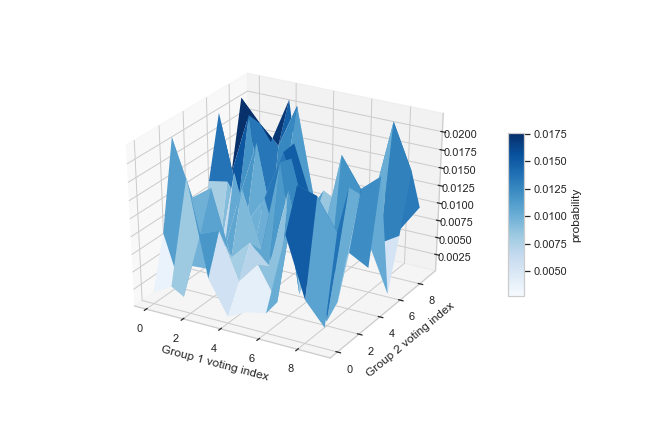
\includegraphics[width=\linewidth]{figures/2d_viz.png}
 \caption{Distribution of Probability over the 2D Hypercube for a Model in the $2 \times 2$ Case}
 \label{fig:2d_viz}
\end{figure}

Figure \ref{fig:3d_viz} shows the distribution of probability over the $2$D hypercube for a model in the $3 \times 2$ case. Since there are $3$ dimensions for demographic groups, Figure \ref{fig:3d_viz} presents the fourth dimension, probability, as directed arrows across a cross section of the dimensions. The colors of these arrows give the corresponding probability.

\begin{figure}[ht]\centering
 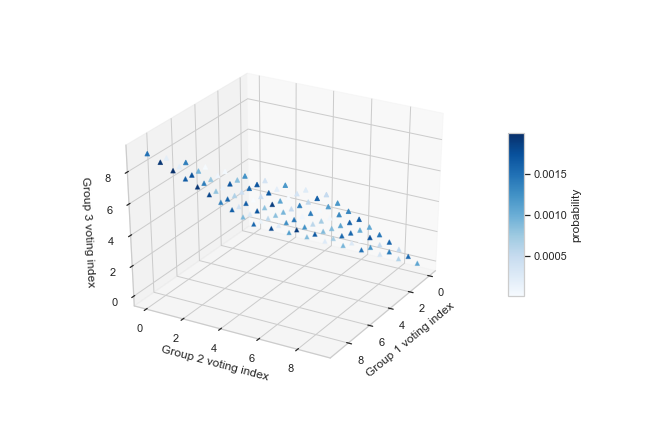
\includegraphics[width=\linewidth]{figures/3d_viz.png}
 \caption{Distribution of Probability over the 3D Hypercube for a Model in the $3 \times 2$ Case}
 \label{fig:3d_viz}
\end{figure}
